\documentclass{article}\usepackage[]{graphicx}\usepackage[]{color}
%% maxwidth is the original width if it is less than linewidth
%% otherwise use linewidth (to make sure the graphics do not exceed the margin)
\makeatletter
\def\maxwidth{ %
  \ifdim\Gin@nat@width>\linewidth
    \linewidth
  \else
    \Gin@nat@width
  \fi
}
\makeatother

\definecolor{fgcolor}{rgb}{0.345, 0.345, 0.345}
\newcommand{\hlnum}[1]{\textcolor[rgb]{0.686,0.059,0.569}{#1}}%
\newcommand{\hlstr}[1]{\textcolor[rgb]{0.192,0.494,0.8}{#1}}%
\newcommand{\hlcom}[1]{\textcolor[rgb]{0.678,0.584,0.686}{\textit{#1}}}%
\newcommand{\hlopt}[1]{\textcolor[rgb]{0,0,0}{#1}}%
\newcommand{\hlstd}[1]{\textcolor[rgb]{0.345,0.345,0.345}{#1}}%
\newcommand{\hlkwa}[1]{\textcolor[rgb]{0.161,0.373,0.58}{\textbf{#1}}}%
\newcommand{\hlkwb}[1]{\textcolor[rgb]{0.69,0.353,0.396}{#1}}%
\newcommand{\hlkwc}[1]{\textcolor[rgb]{0.333,0.667,0.333}{#1}}%
\newcommand{\hlkwd}[1]{\textcolor[rgb]{0.737,0.353,0.396}{\textbf{#1}}}%
\let\hlipl\hlkwb

\usepackage{framed}
\makeatletter
\newenvironment{kframe}{%
 \def\at@end@of@kframe{}%
 \ifinner\ifhmode%
  \def\at@end@of@kframe{\end{minipage}}%
  \begin{minipage}{\columnwidth}%
 \fi\fi%
 \def\FrameCommand##1{\hskip\@totalleftmargin \hskip-\fboxsep
 \colorbox{shadecolor}{##1}\hskip-\fboxsep
     % There is no \\@totalrightmargin, so:
     \hskip-\linewidth \hskip-\@totalleftmargin \hskip\columnwidth}%
 \MakeFramed {\advance\hsize-\width
   \@totalleftmargin\z@ \linewidth\hsize
   \@setminipage}}%
 {\par\unskip\endMakeFramed%
 \at@end@of@kframe}
\makeatother

\definecolor{shadecolor}{rgb}{.97, .97, .97}
\definecolor{messagecolor}{rgb}{0, 0, 0}
\definecolor{warningcolor}{rgb}{1, 0, 1}
\definecolor{errorcolor}{rgb}{1, 0, 0}
\newenvironment{knitrout}{}{} % an empty environment to be redefined in TeX

\usepackage{alltt}
%\usepackage[utf8]{inputenc}

\title{Title}
\author{Author Name}
\date{Date}

\usepackage{amsmath,amsfonts,amssymb}
\usepackage{natbib}
\usepackage{graphicx}
\IfFileExists{upquote.sty}{\usepackage{upquote}}{}
\begin{document}

\maketitle

\section{Introduction}
There is a theory which states that if ever anyone discovers exactly what the Universe is for and why it is here, it will instantly disappear and be replaced by something even more bizarre and inexplicable.
There is another theory which states that this has already happened.

\begin{figure}[h!]
\centering
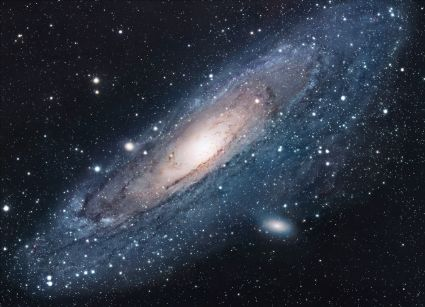
\includegraphics[scale=1.7]{universe}
\caption{The Universe}
\label{fig:universe}
\end{figure}

\section{Using R Code}

We should load all of the libraries that we will use. 
\begin{knitrout}
\definecolor{shadecolor}{rgb}{0.969, 0.969, 0.969}\color{fgcolor}\begin{kframe}
\begin{alltt}
\hlkwd{library}\hlstd{(tidyverse)}
\end{alltt}
\end{kframe}
\end{knitrout}

Now with our libraries loaded we can use their functions. Let's import some data and produce a plot. 
\begin{knitrout}
\definecolor{shadecolor}{rgb}{0.969, 0.969, 0.969}\color{fgcolor}\begin{kframe}
\begin{alltt}
\hlstd{df} \hlkwb{<-} \hlkwd{read_csv}\hlstd{(}\hlstr{"Data/sampleData.csv"}\hlstd{)}
\end{alltt}
\end{kframe}
\end{knitrout}

Before we make a plot, we should take a brief look at our data and perhaps compute some very simple descriptive statistics. 

Here are the first five rows of our data:
\begin{knitrout}
\definecolor{shadecolor}{rgb}{0.969, 0.969, 0.969}\color{fgcolor}\begin{kframe}
\begin{alltt}
\hlkwd{head}\hlstd{(df,}\hlnum{5}\hlstd{)}
\end{alltt}
\begin{verbatim}
## # A tibble: 5 x 5
##   student    id color defect total.number
##   <chr>   <int> <chr> <chr>         <int>
## 1 daceyij     1 BR    N                57
## 2 daceyij     2 O     N                57
## 3 daceyij     3 BL    N                57
## 4 daceyij     4 G     L                57
## 5 daceyij     5 BL    N                57
\end{verbatim}
\end{kframe}
\end{knitrout}

We can get a simple summary of our data:
\begin{knitrout}
\definecolor{shadecolor}{rgb}{0.969, 0.969, 0.969}\color{fgcolor}\begin{kframe}
\begin{alltt}
\hlkwd{summary}\hlstd{(df)}
\end{alltt}
\begin{verbatim}
##    student                id           color              defect         
##  Length:4777        Min.   : 0.00   Length:4777        Length:4777       
##  Class :character   1st Qu.:14.00   Class :character   Class :character  
##  Mode  :character   Median :28.00   Mode  :character   Mode  :character  
##                     Mean   :27.68                                        
##                     3rd Qu.:41.00                                        
##                     Max.   :59.00                                        
##   total.number  
##  Min.   :47.00  
##  1st Qu.:53.00  
##  Median :55.00  
##  Mean   :54.38  
##  3rd Qu.:56.00  
##  Max.   :59.00
\end{verbatim}
\end{kframe}
\end{knitrout}

Now let's create a bar plot:
\begin{knitrout}
\definecolor{shadecolor}{rgb}{0.969, 0.969, 0.969}\color{fgcolor}\begin{kframe}
\begin{alltt}
\hlkwd{ggplot}\hlstd{(}\hlkwc{data}\hlstd{=df,}\hlkwc{mapping} \hlstd{=} \hlkwd{aes}\hlstd{(}\hlkwc{x}\hlstd{=color,}\hlkwc{y}\hlstd{=total.number))} \hlopt{+}
  \hlkwd{geom_bar}\hlstd{(}\hlkwc{stat}\hlstd{=}\hlstr{"identity"}\hlstd{)}
\end{alltt}
\end{kframe}
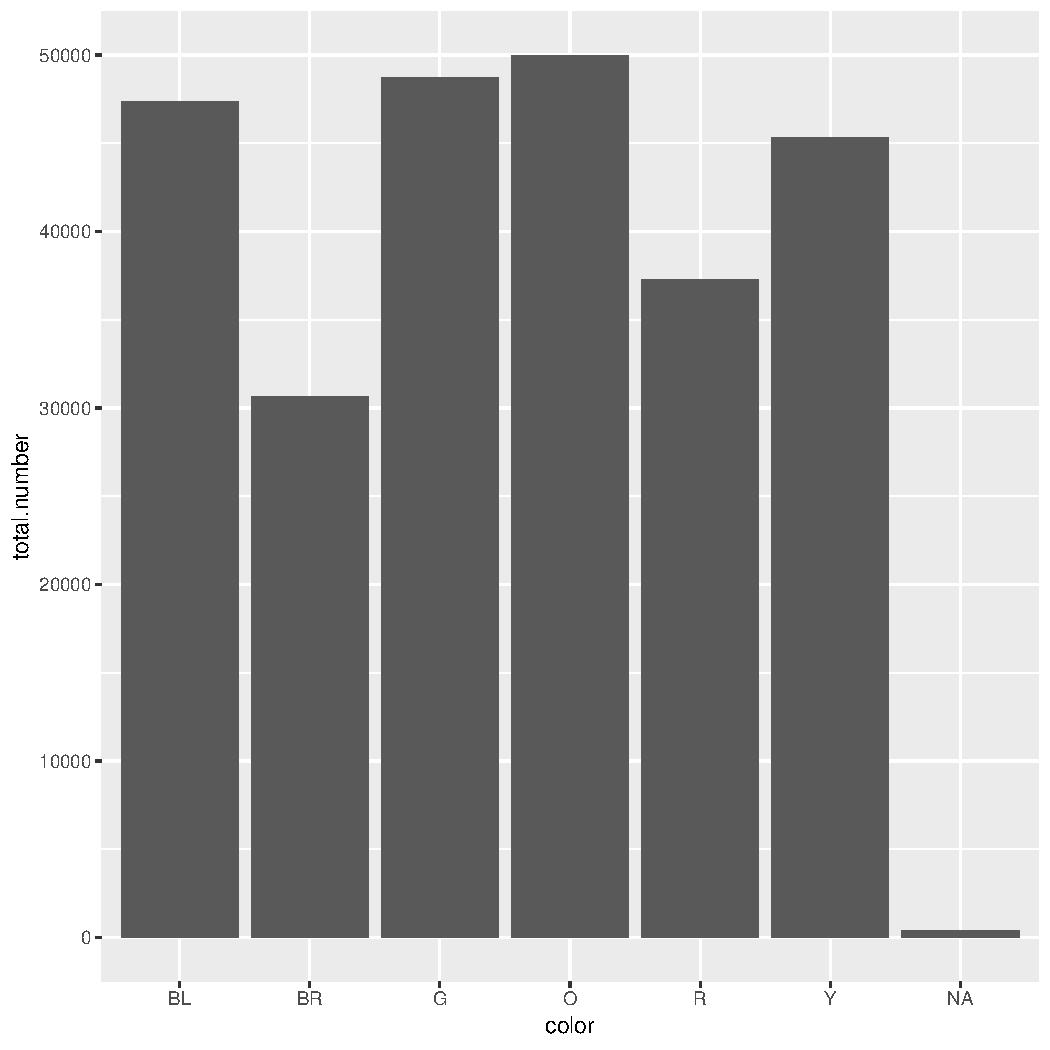
\includegraphics[width=\maxwidth]{figure/unnamed-chunk-5-1} 

\end{knitrout}

\section{Mathematics}

Here is how you can typeset some mathematics in \LaTeX. Inline uses dollar signs $y = mx + b$. You can also give an expression its own line
\[ y = \frac{1}{2}x + 10. \]
Some symbols have their own command. For example, you can produce a Greek letter like this $\alpha$. 

A lot of notation is possible with \LaTeX. For example, 
\[ \frac{d}{dx}x^2 = 2x,  \]
and
\[ \int_{0}^{1}x\ dx = \frac{1}{2}. \]

\section{Conclusion}
``I always thought something was fundamentally wrong with the universe'' \citep{adams1995hitchhiker}

\bibliographystyle{plain}
\bibliography{references}
\end{document}
